\documentclass[11pt,fleqn]{article}
\usepackage{pgf,tikz}
\usepackage[ngerman]{babel}
\usepackage[utf8]{inputenc}
\usepackage[T1]{fontenc}
\usepackage{float}
\usepackage{mathtools}
\usepackage{fancyhdr}
\usepackage[margin=1.2in]{geometry}
\usepackage{graphicx}
\usepackage{lmodern}
\usepackage{circuitikz}
\usepackage{pgfplots}
\usepackage{pgfplotstable}
\usepackage{amsmath}
\usepackage{amssymb}
\usepackage{amsfonts}
\usepackage{siunitx}
\usepackage[backend=biber, citestyle=alphabetic, style=alphabetic]{biblatex}
\usepackage{pdfpages}


\bibliography{literatur.bib}

\parindent 0pt
\parskip 10pt
\newcommand{\degre}{\ensuremath{^\circ}}

\title{Technische Optik \\ Praktikum Laser-Triangulation}
\date{09. Juli 2015}
\author{Hans Herrmann \and Felix Kayser \and Hermann Pommerenke \and Tino Steinmetz}

\begin{document}
	\pagenumbering{gobble}
	\begin{figure}[t]
	    \centering
	    
\includegraphics[width=115mm]{img/UNI-Logo_Siegel_4c_115mm_07.png}
	\end{figure}

	\maketitle
	
	\thispagestyle{empty}

	\newpage
	\pagenumbering{Roman}
	\pagestyle{headings}
	\tableofcontents
	
	\everymath{\displaystyle} % Jede Formel im Displaystyle
	
	\newpage
	\pagenumbering{arabic}

	\section{Einleitung}

\subsection{Prinzip der Laser-Triangulation}

Die Laser-Triangulation ist ein Verfahren zur optischen Abstandsmessung. Dabei wird die Eigenschaft einer Linse genutzt, den Winkel eines einfallenden Lichtstrahls in den Ort eines auf einen Schirm projizierten Bildpunktes zu transformieren. Bei dem erfassten Lichtstrahl handelt es sich dabei um den Lichtpunkt eines Lasers, der ein Objekt trifft. Der Projektionsschirm wird durch den CCD-Sensor einer Kamera gebildet.

Wird das Objekt entlang des Laserstrahls verschoben, so ändert sich auch der Einfallswinkel auf das Linsensystem der feststehenden Kamera und es kommt zu einer Verschiebung des Bildpunktes auf dem Sensor. Aus dieser Verschiebung kann dann auf die Entfernungsänderung des Objektes geschlossen werden.

\begin{figure}[h!]
	\centering
	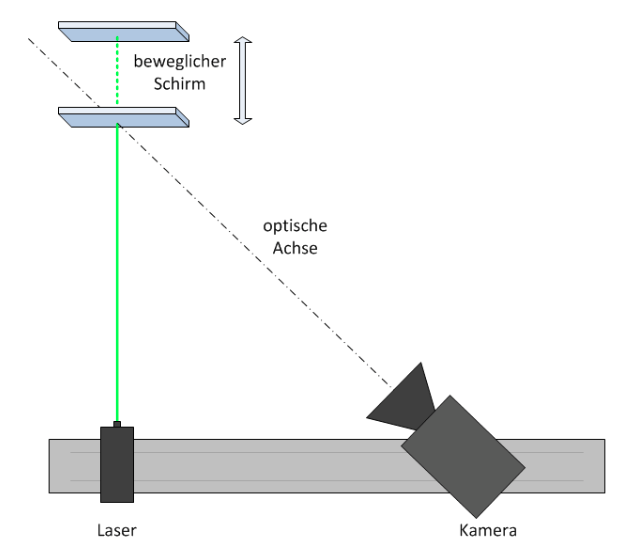
\includegraphics[width=0.8\linewidth]{img/Lasertriangulation_schema}
	\caption{Schematischer Versuchsaufbau \cite{versuchsanleitung_lasertriangulation}}
	\label{fig:schema_aufbau}
\end{figure}

\subsection{Herleitung}

In diesem Abschnitt erfolgt die Herleitung der Formel, durch die aus dem Abstand der Projektionen auf dem CCD-Sensor die Entfernungsänderung des Schirms berechnet werden kann. Die verwendeten Größen können Abbildung~\ref{fig:geometrie} entnommen werden.

Die zurückgelegte Entfernung ergibt sich aus der Differenz der Gesamtentfernung $z_{ges}$ und des Startpunktes $z_0$.
\begin{equation}
	z = z_{ges} - z_0
	\label{eq:z1}
\end{equation}
Da sich die Strahlengänge in rechtwinklige Dreiecke unterteilen lassen, können durch Anwendung des Cosinus- und Sinussatzes Ausdrücke für $z_{ges}$ und $z_0$ bestimmt werden, die nur von der Entfernung $d$ zwischen Linse und Laser und den Winkeln $\alpha$ und $\beta$ abhängen.
\begin{align}
	\left.\begin{aligned}
		\cos(\beta-\alpha) &= \frac{z_{ges}}{g'}\\
		\sin(\beta-\alpha) &= \frac{d}{g'}
	\end{aligned}\qquad\right\}\qquad z_{ges} &= d\cdot\frac{\cos(\beta-\alpha)}{\sin(\beta-\alpha)}\\[1em]
	\left.\begin{aligned}
		\cos(\beta) &= \frac{z_0}{g_1}\\ 
		\sin(\beta) &= \frac{d}{g_1}
	\end{aligned}\qquad\right\}\qquad z_0 &= d\cdot\frac{\cos(\beta)}{\sin(\beta)}
\end{align}
Die entstandenen Terme können nun in Gleichung~(\ref{eq:z1}) eingesetzt werden. Wie man leicht sieht lassen sich die Brüche der Winkelfunktionen in den Cotangens überführen. 
\begin{align}
	z &= d\cdot\left(\frac{\cos(\beta-\alpha)}{\sin(\beta-\alpha)}-\frac{\cos(\beta)}{\sin(\alpha)}\right)\\
	  &= d\cdot\left(\cot(\beta-\alpha)-\cot(\beta)\right)
	  \label{eq:z2}
\end{align}
Da der Winkel $\alpha$ nicht direkt gemessen werden kann muss ein Ausdruck gefunden werden, der von den Parametern des Optischen Systems abhängt. Dazu werden zunächst die Punktverschiebung auf dem CCD-Sensor $\Delta p'$ und die Bildweite $b$ als bekannt angenommen.
\begin{equation}
	\left.\begin{aligned}
		\sin(\alpha) &= \frac{\Delta p'}{b'}\\
	\cos(\alpha) &= \frac{b}{b'}
	\end{aligned}\qquad\right\}\qquad
	\frac{\sin(\alpha)}{\cos(\alpha)} = \frac{\Delta p'}{b} = \tan(\alpha)
\end{equation}
Durch Umkehrung des Tangens erhält man nun für $\alpha$:
\begin{equation}
	\alpha = \arctan\left(\frac{\Delta p'}{b}\right)
	\label{eq:alpha}
\end{equation}
Da auch der Abstand $d$ zwischen Brennpunkt und Laser nicht genau bestimmt werden kann, ist es notwendig diesen durch bekannte Größen zu substituieren. Abhilfe schafft hier die Anwendung des Sinussatzes auf den Winkel $\beta$.
\begin{align}
	\sin(\beta) &= \frac{d}{g_1}\\
	d &= g_1\cdot\sin(\beta)
	\label{eq:d}
\end{align}
Setzt man nun (\ref{eq:alpha}) und (\ref{eq:d}) in Gleichung~(\ref{eq:z2}) ein, so ergibt sich folgender Ausdruck:
\begin{equation}
	z = g_1\cdot\sin(\beta)\cdot\left\{\cot\left[\beta-\arctan\left(\frac{\Delta p'}{b}\right)\right]-\cot(\beta)\right\}
	\label{eq:z3}
\end{equation}
Mit Hilfe der Linsengleichung (\ref{eq:linsengleichung}) muss nun noch ein passender Ausdruck für $b$ gefunden werden.
\begin{align}
	\frac{1}{f} &= \frac{1}{b} + \frac{1}{g} \label{eq:linsengleichung}\\
	b &= \frac{f\cdot g}{g-f} \label{eq:b}
\end{align}
Durch das Einsetzen von (\ref{eq:b}) in Gleichung~(\ref{eq:z3}) ergibt sich ein Ausdruck für $z$, der nur von bekannten oder messbaren Größen abhängt. 
\begin{equation}
	z = g_1\cdot\sin(\beta)\cdot\left\{\cot\left[\beta-\arctan\left(\frac{\Delta p'(g-f)}{fg}\right)\right]-\cot(\beta)\right\}
	\label{eq:zfinal}
\end{equation}

\begin{figure}[h]
	\centering
	\begin{tikzpicture}[scale=0.8]
		\draw (0,0) -- (10,0) -- (10,3) coordinate (a3);
		% Laser
		\draw[green!90!black, thick] (0,0) -- (0,10);
		\draw[red, thick, dashed] (0,10) -- (0,12);
		% gestrichelte Linie
		\draw[dash dot] (12.5,-2.5) coordinate (a6) -- (10,0);
		\draw[dash dot] (10,0) coordinate (a2) -- (0,10) coordinate (a1);
		\draw[dash dot]	(0,10) -- (-1,11);
		% blau gestrichelte Linie
		\draw[dash dot, blue] (10,0) -- (0,12) coordinate (a4);
		\draw[dash dot, blue] (12.27,-2.72) coordinate (a7) -- (10,0);
		% Sensor und Schärfeebene
		\draw (-1,11) coordinate (a5) -- (0,12);
		\draw (11.5,-3.5) -- (13.5,-1.5);
		% Winkelbezeichnungen
		\draw pic["$\beta$", draw=black, angle eccentricity=0.8, angle radius=2cm]{angle=a3--a2--a1};
		\draw pic["$\alpha$", draw=black, angle eccentricity=0.95, angle radius=7cm]{angle=a4--a2--a1};
		\draw pic["$\cdot$", draw=black, angle eccentricity=0.5, angle radius=0.3cm]{angle=a1--a5--a4};	
		\draw pic["$\cdot$", draw=black, angle eccentricity=0.5, angle radius=0.2cm]{angle=a2--a6--a7};
		% Beschriftungen
		\draw (5,5) node[anchor=north east]{$g_1$};
		\draw (-0.5,10.5) node[anchor=north east]{$g_2$};
		\draw (0,11) node[anchor=west, red]{$z$};
		\draw (-0.5,11.5) node[anchor=south east]{$\Delta p$};
		\draw (5,6) node [anchor=south west, blue]{$g'$};
		\draw (11.25,-1.25) node [anchor=south west]{$b$};
		\draw (11.1,-1.4) node [anchor=north east, blue]{$b'$};
		\draw (12.4,-2.6) node [anchor=north west]{$\Delta p'$};
		\draw (13.5,-1.5) node [anchor=west]{CCD-Sensor};
		\draw (0,5) node[anchor=west, green!90!black]{$z_0$};
	\end{tikzpicture}
	\caption{geometrisch Darstellung der Strahlengänge}
	\label{fig:geometrie}
\end{figure}
	
	\clearpage
	\section{Versuchsaufbau}

\begin{figure}[h!]
	\centering
	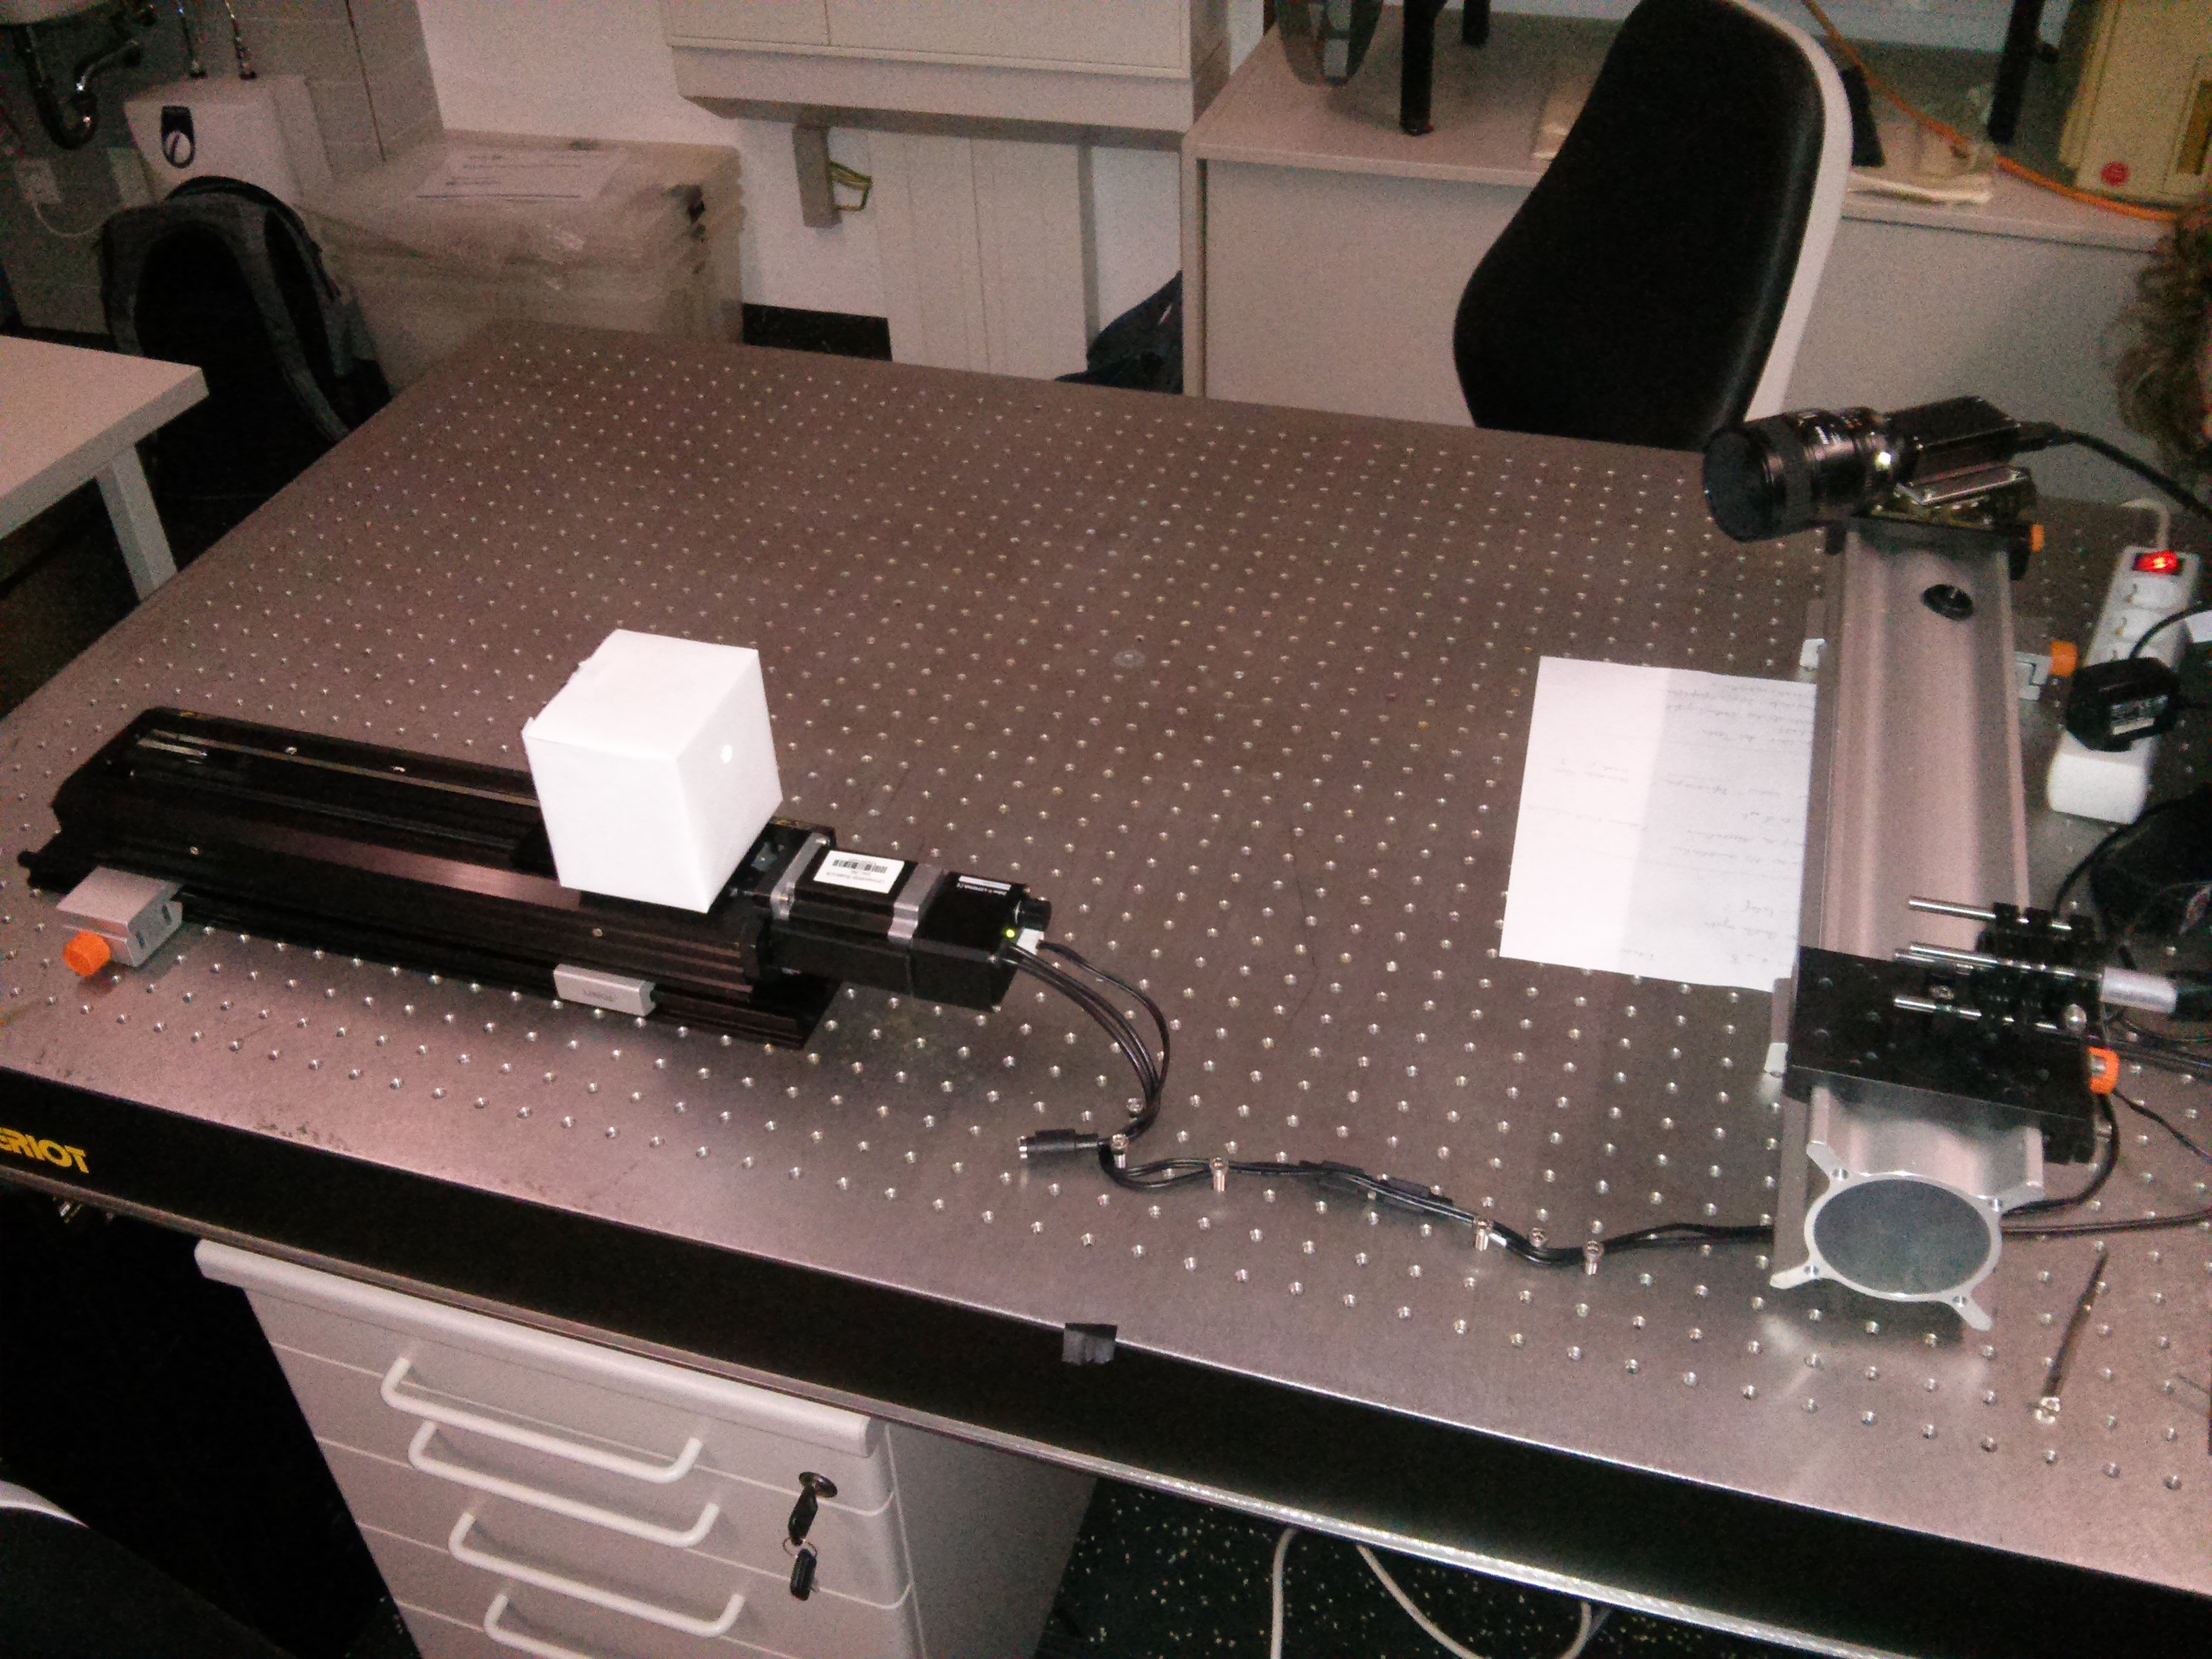
\includegraphics[width=0.8\linewidth]{img/versuchsaufbaufoto.jpg}
	\caption{Versuchsaufbau}
	\label{fig:Versuchsaufbau}
\end{figure}

Der Versuchsaufbau bestand aus insgesamt drei voneinander örtlich getrennten Komponenten. 

Die Komponenten des zu vermessenden Systems, bestehend aus einem grünen $\SI{532}{\nm}$ Laser (Neodym-dotierter Yttrium-Aluminium-Granat-Laser (Nd:YAG)) und einem Messobjekt, sind in einer Linie angeordnet. Dieses Messobjekt hat die Form eines Würfels. Die Oberfläche dieses Würfels ist mit weißem Papier umspannt, um den Laserpunkt gutsichtbar abzubilden. Der Würfel konnte mittels einer Linearachse (Zaber T-LST0250 A) mit einer Genauigkeit von $0.124023438 \si{\micro\meter}$ in z-Richtung verschoben werden. Der Schrittmotor der Linearachse konnte mithilfe des angeschlossenen PCs angesteuert werden.

Das beobachtende System bestand aus einer Kamera (Basler Scout scA1400-36fm) mit einem $\SI{60}{\mm}$ Nikon Objektiv. Die erfassten Bilder wurden direkt an den angeschlossenen PC zur weiteren Verarbeitung übertragen.

Die Auswertung der im Versuch aufgenommenen Bilder erfolgte auf einem direkt an die Komponenten des Versuchsaufbaus angeschlossenen PCs mithilfe der Software Mathcad.

Um auf den aufgenommenen Bildern Störlichtquellen abzuschirmen musste Tino dauerhaft vor einer Steckerleiste stehen, bis er diese einfach abschaltete $\ddot\smile$

\emph{Ja, das lassen wir vllt eher nicht drin \ldots}
	
	\clearpage
	\section{Auswertung}

Die Abb.  \ref{fig:00mm} und \ref{fig:10mm} zeigen die von der Kamera aufgenommenen Bilder beispielhaft für die Extrempositionen der gemessenen Verschiebung. Da die Reflexion eines Lasers nicht in einem Punkt lokalisiert ist, wurde die genaue Position der Abbildung auf dem Kamerasensor vergleichend mittels zwei verschiedener Verfahren ermittelt.

Für beide Verfahren wurde zunächst die Intensität spaltenweise aufsummiert.

Die einfachere Variante ermittelte nun die Position $px_m$ auf dem CCD-Sensor in Pixeln  durch Auswahl der Spalte mit der größten Intensitätssumme als Zentrum des Laserpunkts. Die Genauigkeit dieses Verfahrens ist folglich gleich oder kleiner der Sensorauflösung, die Pixelangabe somit ganzzahlig.

Alternativ wurde die Position subpixelgenau über eine Regression ermittelt. Hierfür wurde die Intensitätsverteilung des Lasers als gaußförmig angenommen. In der logarithmiertem Darstellung entspricht das einer Parabel, für welche eine Regression leicht durchgeführt werden kann. Der Scheitelpunkt dieser Parabel wurde als Position $px_g$ in Pixeln verwendet. Dieses Verfahren kann die Position mit einer Genauigkeit über der Pixelauflösung bestimmen.

Die so bestimmte Pixelposition entspricht (nach Differenzbildung mit einem Referenzpunkt, in diesem Fall $z=0$) gemäß Gl. (\ref{eq:zfinal}) einer $z$-Verschiebung $z_m$ bzw. $z_g$.

In Tab. \ref{tab:messwerte} sind die ermittelten Größen ersichtlich.

Zum Vergleich der beiden Verfahren wurden aus ermittelter und bekannter (da eingestellter) Verschiebung die absoluten $\Delta z_{m,g}$ und relativen Fehler $|\Delta z_{m,g}/z|$ für jedes der Wertetupel errechnet. Man erkennt schnell, dass das Regressionsverfahren nicht nur subpixelgenau ist, sondern auch viel geringere stochastische Fehler macht. Es zeigt bezüglich der Intensitätsverteilung Tiefpassverhalten. Der in Abb. \ref{fig:plot_rel} ersichtliche Verlauf des Fehlers ist vorhersehbar und kann folglich bei bekanntem Messaufbau herausgerechnet werden, was die Genauigkeit noch weiter steigert.

Zusammenfassend ist das Gaußkurven-Regressionsverfahren somit besser geeignet, wenn Ortsbestimmung sehr genau erfolgen muss. Es erfordert jedoch auch eine deutlich höhere Rechenleistung. Daher hat das Maximalwertsverfahren die bessere Echtzeitfähigkeit.

\begin{figure}[tbh]
	\centering
	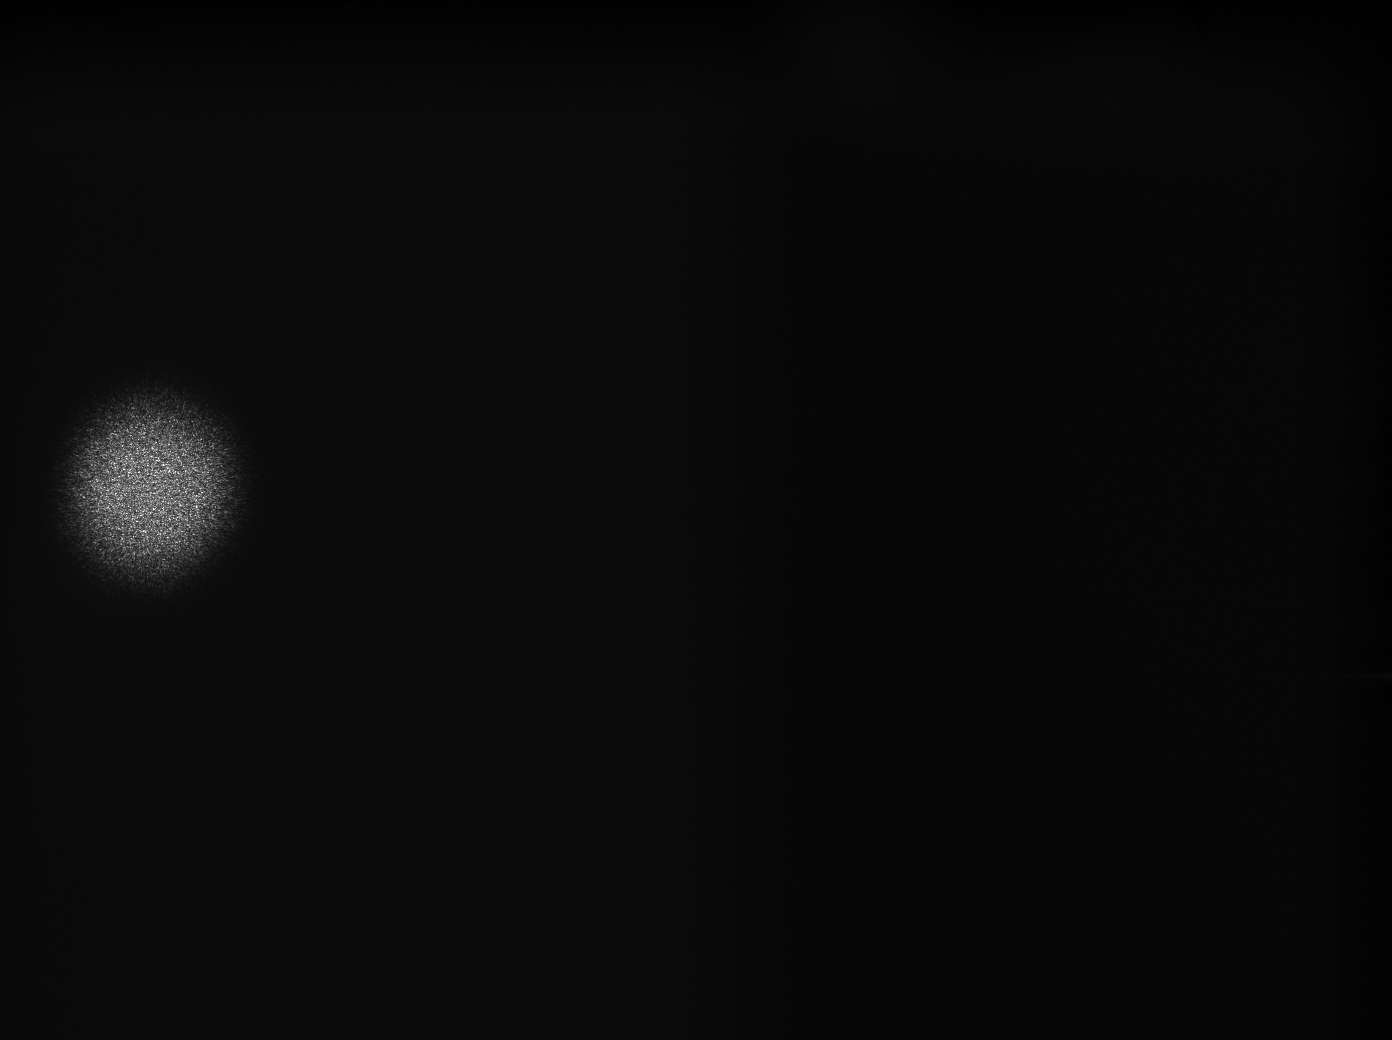
\includegraphics[width=0.8\linewidth]{img/00cm.jpg}
	\caption{Aufnahme für $z=0$}
	\label{fig:00mm}
\end{figure}

\begin{figure}[tbh]
	\centering
	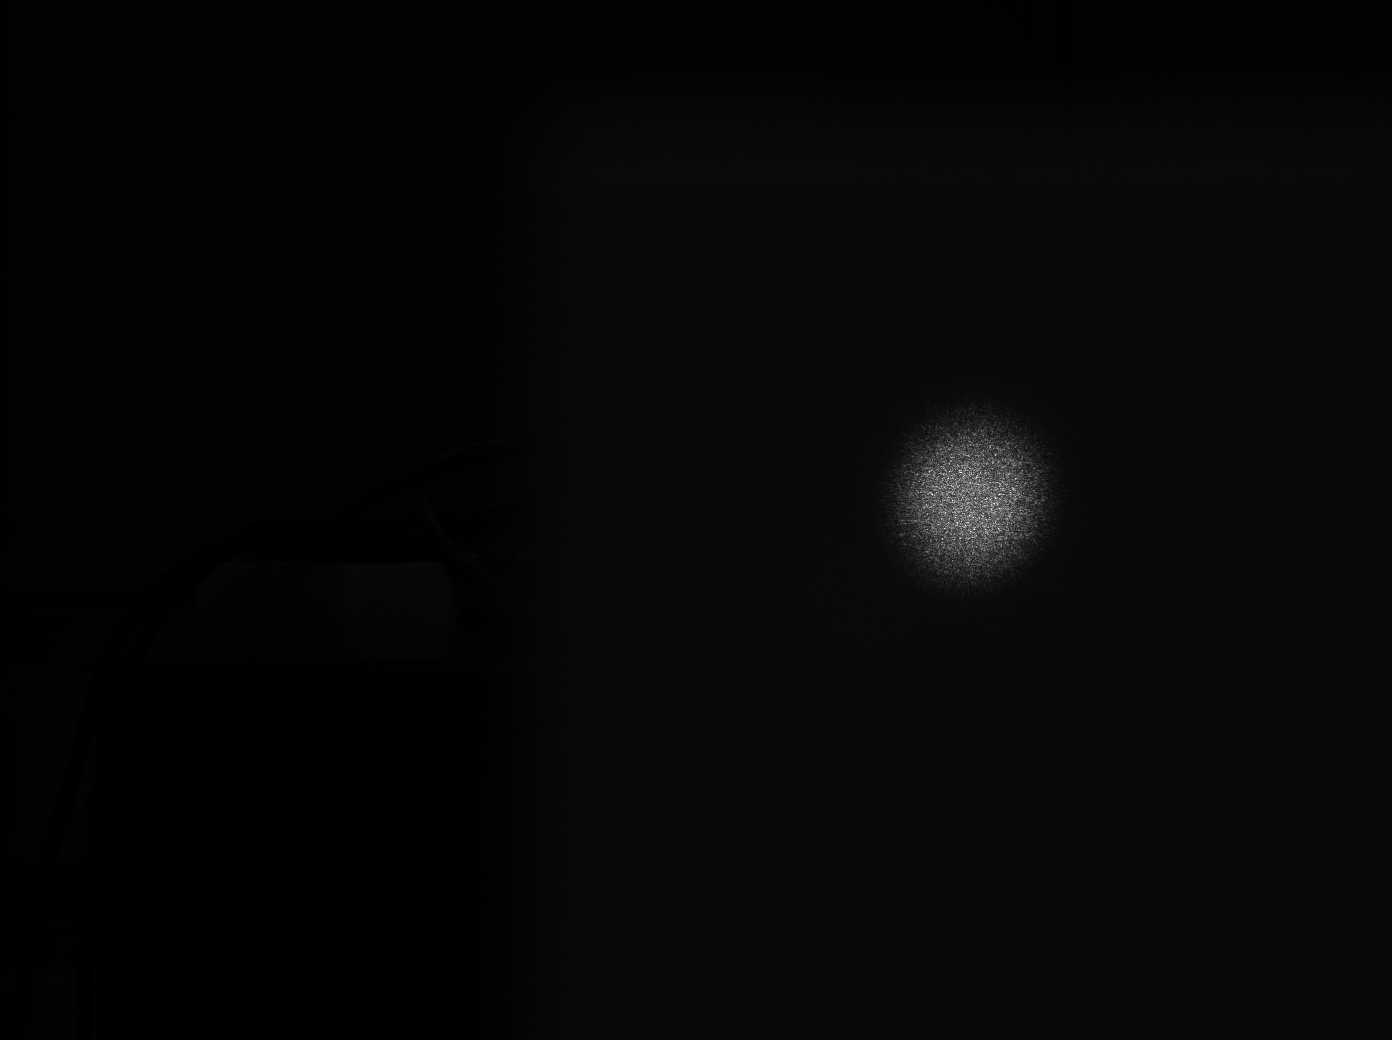
\includegraphics[width=0.8\linewidth]{img/100cm.jpg}
	\caption{Aufnahme für $z=\SI{10}{\mm}$}
	\label{fig:10mm}
\end{figure}

\begin{table}[tbh]
	\centering
	\pgfplotstabletypeset[
	col sep=comma,
	precision = 2,
	fixed,
	dec sep align,
	every head row/.style={,after row=\hline},
	every last row/.style={after row=\hline},
	columns={d,png,pnm,dg,dm,afg,afm,rfg,rfm},
	columns/d/.style={column name=$z/\si{\milli\meter}$},
	columns/png/.style={column name=$px_g$},
	columns/pnm/.style={column name=$px_m$},
	columns/dg/.style={column name=$z_g/\si{\milli\meter}$},
	columns/dm/.style={column name=$z_m/\si{\milli\meter}$},
	columns/afg/.style={column name=$\Delta z_g/\si{\milli\meter}$},
	columns/afm/.style={column name=$\Delta z_m/\si{\milli\meter}$},
	columns/rfg/.style={column name=$|\Delta z_g/z|/\%$},
	columns/rfm/.style={column name=$|\Delta z_m/z|/\%$},	
	]{./tab/Triangulation.csv}
	\caption{Messwerte}
	\label{tab:messwerte}
\end{table}

\begin{figure}[tbh]
	\centering
	\begin{tikzpicture}[trim axis left, trim axis right]
	\begin{axis}[width=0.9\textwidth,
	height=0.35\textheight,
	%y label style = {rotate=-90},
	%y tick label style={/pgf/number format/.cd,fixed, fixed zerofill},
	%x tick label style={/pgf/number format/.cd,fixed, fixed zerofill},
	grid=both,                     
	%title={Der Titel}, 
	xlabel={$z/\si{\milli\meter}$}, 
	ylabel={Absolute Fehler in $\si{\milli\meter}$},
	ybar,
	bar width = 7pt,
	xmin=-5,
	xmax=105,
	%ymin=0,
	%ymax=4,
	%xtick={0,0.2,0.4,0.6,0.8,1},
	legend pos = south east,
	legend cell align = left,
	legend entries={$\Delta z_g$, $\Delta z_m$}
	]                
	%\addlegendimage{mark=*, color=red}
	%\addlegendimage{mark=*, color=blue}     
	\addplot[blue, fill] table[x=d, y=afg, col sep=comma]{./tab/Triangulation.csv};
	\addplot[red, fill] table[x=d, y=afm, col sep=comma]{./tab/Triangulation.csv};
	\end{axis}
	\end{tikzpicture}
	\caption{Absolute Fehler}
	\label{fig:plot_abs}
\end{figure}

\begin{figure}[tbh]
	\centering
	\begin{tikzpicture}[trim axis left, trim axis right]
	\begin{axis}[width=0.9\textwidth,
	height=0.35\textheight,
	%y label style = {rotate=-90},
	%y tick label style={/pgf/number format/.cd,fixed, fixed zerofill},
	%x tick label style={/pgf/number format/.cd,fixed, fixed zerofill},
	grid=both,                     
	%title={Der Titel}, 
	xlabel={$z/\si{\milli\meter}$}, 
	ylabel={Relativer Fehler in $\%$},
	ybar,
	bar width = 7pt,
	xmin=-5,
	xmax=105,
	ymin=0,
	%ymax=4,
	%xtick={0,0.2,0.4,0.6,0.8,1},
	legend pos = north east,
	legend cell align = left,
	legend entries={$|\Delta z_g/z|$, $|\Delta z_m/z|$}
	]                
	%\addlegendimage{mark=*, color=red}
	%\addlegendimage{mark=*, color=blue}     
	\addplot[yellow!90!black, fill] table[x=d, y=rfg, col sep=comma]{./tab/Triangulation.csv};
	\addplot[green!60!black, fill] table[x=d, y=rfm, col sep=comma]{./tab/Triangulation.csv};
	\end{axis}
	\end{tikzpicture}
	\caption{Relative Fehler}
	\label{fig:plot_rel}
\end{figure}
	
	\clearpage
	\printbibliography
\end{document}
